
%%%%%%%%%%%%%%%%%%%%%%% file typeinst.tex %%%%%%%%%%%%%%%%%%%%%%%%%
%
% This is the LaTeX source for the instructions to authors using
% the LaTeX document class 'llncs.cls' for contributions to
% the Lecture Notes in Computer Sciences series.
% http://www.springer.com/lncs       Springer Heidelberg 2006/05/04
%
% It may be used as a template for your own input - copy it
% to a new file with a new name and use it as the basis
% for your article.
%
% NB: the document class 'llncs' has its own and detailed documentation, see
% ftp://ftp.springer.de/data/pubftp/pub/tex/latex/llncs/latex2e/llncsdoc.pdf
%
%%%%%%%%%%%%%%%%%%%%%%%%%%%%%%%%%%%%%%%%%%%%%%%%%%%%%%%%%%%%%%%%%%%


\documentclass[runningheads,a4paper]{llncs}

\usepackage{amssymb}
\setcounter{tocdepth}{3}
\usepackage{graphicx}

\usepackage{url}
\urldef{\mailsa}\path|{caldwelt, david.t.coleman, nikolaus.correll}@colorado.edu|    
\newcommand{\keywords}[1]{\par\addvspace\baselineskip
\noindent\keywordname\enspace\ignorespaces#1}

\usepackage{color}

\begin{document}

\mainmatter  % start of an individual contribution

% first the title is needed
\title{Robotic Manipulation for Identification of Flexible Object}

% a short form should be given in case it is too long for the running head
\titlerunning{Robotic Manipulation for Identification of Flexible Object}


\author{T. M. Caldwell and  D. Coleman and N. Correll%
\thanks{
This work was supported by a NASA
Early Career Faculty fellowship NNX12AQ47GS02. We are grateful for this support.}%
}
%
\authorrunning{Robotic Manipulation for Identification of Flexible Object}
% (feature abused for this document to repeat the title also on left hand pages)

% the affiliations are given next; don't give your e-mail address
% unless you accept that it will be published
\institute{Department of Computer Science, University of Colorado,\\
1111 Engineering Dr, Boulder, CO 80309, USA\\
\mailsa}

\toctitle{Lecture Notes in Computer Science}
\tocauthor{Authors' Instructions}
\maketitle

\section{Motivation, Problem Statement, Related Work} 
\begin{figure}
\centering
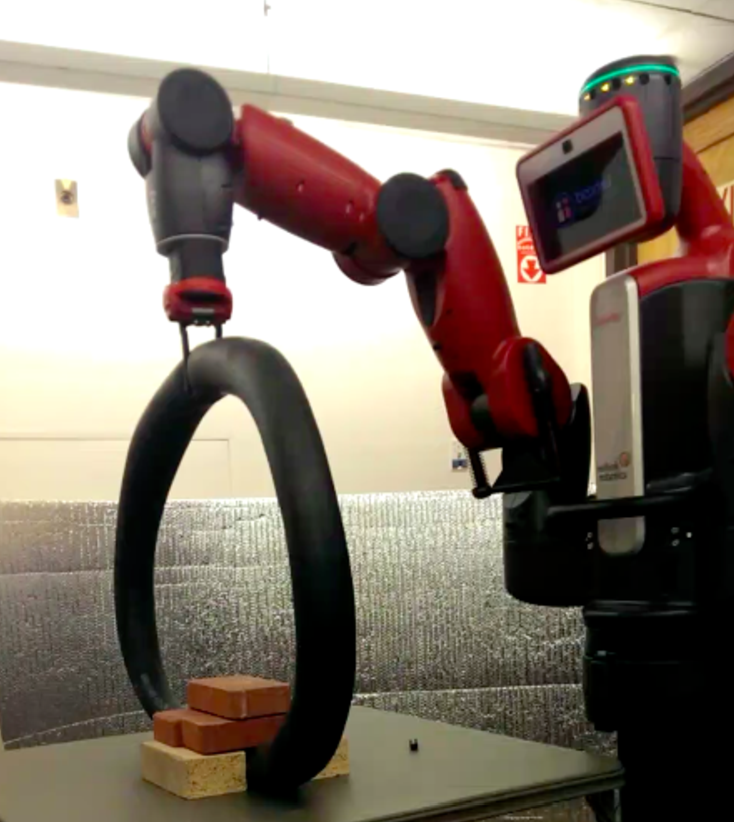
\includegraphics[width = 180pt]{baxter_experiment_image}
\caption{Rethink Robotics' Baxter manipulating an inflated bicycle tyre.}
\label{fig-baxter_image_1}
\end{figure}
\begin{enumerate}
\item I see this paper as a ``roadmap paper''.  Sort of these are the challenges, this is how we plan to solve them, and there are a lot of interesting problems.
\item Problem statement: ``When a robot initially interacts with a flexible object with unknown properties, the robot must first manipulate the object, possibly in naive, unstructured manner in order to ascertain characteristics for future purpose driven manipulation.''
\item Proper identification has a number of challenges:
\begin{enumerate}
  \item Integrate touch with visual sensors.
  \item Where/how to initially grip the object.
  \item Multiple grip locations and multiple tests for identification.
  \item Multiple arms.
  \item Additional stimuli like external forces that are due to other objects than the one of consideration---for example, working in a cluttered environment.
  \item Choosing manipulator trajectories that provide the most information.
  \item Unknown topology or geometry
  \item Choosing the model discretization that best balances model fidelity with computation speed.
  \item Stable manipulation while maintaining fidelity of parameter optimization
  \item Updating identification for systems that will change over long time horizon's---for example plant growth over full life cycle.
\end{enumerate}
\item Related Work:
\begin{enumerate}
  \item There are many methods to model and simulate flexible objects \cite{khalil_payeur} \cite{lang_etal}.  A common approach is to model the object as a lattice or collection of links of masses and springs \cite{sahari_etal} \cite{wakamatsu_etal} \cite{khalil_payeur}.
%  \item  Alternatively, the cost can be given by a maximum likelihood estimate for which the cost is lower for parameters that correspond to the simulation that is most consistent with the measurement (see \cite{houska_etal}).  
\end{enumerate}
\item What's new?---``Our approach is similar with the primary difference that the loop connects back onto itself.  This connection restricts the loops movement and is handled using holonomic constraints.  To the best of our knowledge, no one has used a robot to identify parameters of a flexible loop for manipulation.''
\item Who cares?:
\item What difference will it make?---Advancing autonomy of robotic systems.
\item Risks/payoffs?---Additional time and computation to analyze object compared to solely reactive manipulation \textbf{cite}, but once accomplished, model-based planning can be done, which is even more important for potentially unstable manipulation.
\end{enumerate}

\newpage
\section{Technical Approach}
\begin{enumerate}
\item Model based approach---``In this paper, the manner in which we model the loop is so that the underlying mechanics of the loop are the same as the robot arm, i.e., a collection of rigid bodies connected by springs, allowing us to utilize the vast theory of rigid body mechanics \cite{murray_li_sastry}.''
\item Planning and control for full robot/object system---``this enables planning and control to be done in the combined arm and loop configuration space instead of the end effector or object space.''
\item Optimal parameter identification---``optimal control approach for calculating model properties that best match the behavior of the physical loop.''
\begin{enumerate}
\item Setup---``The parameter identification optimization problem is set up as a discrete-time Bolza problem.  For the loop example, the cost functional is a summation of the error between the simulated end effector position and the experimentally-measured end effector position.  The joint error directly correlates to the difference between the simulated loop displacement and the measured loop displacement, at least at the manipulator.''
\item The problem---``For the discrete problem, it is reasonable to choose a discrete cost functional that approximates the continuous cost\textemdash i.e. $\ell_d(x_{k},\rho)\approx\int_{t_{k-1}}^{t_{k}}\ell(x(\tau),\rho)d\tau$ and $m_d(x_{k_f},\rho)\approx m(x(t_f),\rho)$.  Alternatively, $\ell_d$ and $m_d$ can be designed directly without first choosing an underlying continuous cost.  The discrete parameter optimization problem is as follows:
%The integration could be approximated with a quadrature like midpoint rule.  Additionally, in order to use the one-step mapping Eq.(\ref{eq-fk}) and its linerization, Eqs.(\ref{eq-A}) and (\ref{eq-B}), we transform the pair $(q_{k-1},q_k)$ to $(q_k,p_k)=:x_k$ using Eq.(\ref{eq-pk}) so that the discrete running cost instead depends on the state\textemdash i.e. $\ell_d(x_k,\rho)$.  In a similar manner, the discrete terminal cost is chosen to approximate continuous terminal cost\textemdash i.e. $m_d(x_{k_f},\rho)\approx m(x(t_f),\rho)$.  The discrete parameter optimization problem is as follows:
\begin{problem}[Discrete System Parameter Optimization]
Calculate the parameters $\rho\in\mathcal{P}$ which solves:
\[
\min_{\rho\in\mathcal{P}} \Big[J_d(\rho):=\sum_{k=1}^{k_f}\ell_d(x_k,\rho) + m_d(x_{k_f},\rho)\Big]
\]
constrained to $x_{k+1} = f(x_k,\rho,t_k)$, Eq.(\ref{eq-fk}).
\label{prob-disc}
\end{problem}
''
\item The Approach---``In optimal control theory, it is common practice to solve optimization problems using iterative methods.  Iterative optimization methods repeatedly reduce the cost by stepping in a descending direction until a local optimum is found.  Commonly, the step direction and step size is calculated using local derivative information \cite{armijo}\cite{kelley}, which is practiced in this paper.''
\item Gradient---Lemma 1 from paper
\end{enumerate}
\item Using variational integrators---``A good representation of a flexible object is not enough to accurately model it.  We also need the model simulation to be consistent with the physical behavior of the loop.''
\begin{enumerate}
  \item Generalized Coordinates---``Due to recent work by Johnson and Murphey \cite{johnson_murphey_scalable} \cite{johnson_murphey_linearization}, it is possible to efficiently simulate mechanical systems using variational integrators in generalized coordinates. They provide a framework using a tree representation and caching that not only makes for efficient simulation---especially for articulated rigid bodies''
  \item Has good physical properties---``We decided not to apply Euler integration or another low order integrator to the continuous dynamics, as is the case in \cite{sahari_etal}, because such integrators can introduce significant energy errors.  At worst these errors will destabilize the integration and at best compromise the model's energy dissipation \cite{johnson_murphey_scalable}. Instead we decided to use \emph{variational integrators}.  Variational integrators can be used to describe discrete-time equations of motion of a mechanical system.  They are designed from the least action principle and have good properties that agree with known physical phenomenon like stable energy behavior \cite{pekarek_murphey}.''
  \item Holonomic constraints---``variational integrators elegantly handle holonomic constraints.  Holonomic constraints are specified as $h(q) = 0$, where $q$ is the system's configuration.  They are used to constrain positions and orientations.  For the example, we use holonomic constraints to ``close the loop''---i.e. to constrain the link at one end of the loop to the other end.  In simulating continuous dynamics, holonomic constraints are commonly handled with equivalent constraints on the acceleration that can creep due to numerical integration error.  In comparison, variational integrators apply holonomic constraints directly and do not have this issue (see \cite{johnson_murphey_scalable} for a discussion).''
  \item Model based calculations---``efficient model-based calculations like linearizations about a trajectory.   In optimal controls, linearizations are needed for gradient calculations like the gradient calculation presented in this paper.''
\end{enumerate}
\end{enumerate}


\newpage
\section{Results}

\begin{enumerate}
\item Simulation
\item Linearization
\item Gradient calculation
\end{enumerate}


\newpage
\section{Experiments}

At minimum, new experiment grasping rubber tube with both arms.

\begin{figure*}
\centering
\def\svgwidth{.97\textwidth}
\input{three_bloops.pdf_tex}
\caption{Three distinct configurations along with snapshots of the physical system.  \textbf{a)} The frames for Baxter and the loop in their initial configuration. \textbf{b)} Baxter ``twisting'' the loop. \textbf{c)} Baxter ``bending'' the loop.}
\label{fig-3bloops}
\end{figure*}

``We are using a flexible loop as a running example throughout the paper.  We assume the robot has already rigidly grasped the object at one end and that it is clamped at the other. The robot then bends, twists, and stretches the loop.  During the manipulation, the robot measures the arm's joint torques and joint angles.  With this information, it is possible to back out mechanical properties of the loop in order to generate an accurate model for future control and manipulation.''

``The experiment is set up as follows. Baxter’s arm is positioned similarly to that in Figure 1. The top of an inflated rubber loop (bicycle tyre) is placed in Baxter’s gripper and the bottom is clamped to the table. The loop is initially positioned vertically. The loop has a radius of 0.355 meters and a mass of 0.132 kilograms. The arm is run through a recorded motion that is designed to stretch, bend, and twist the tube. The arm’s joint angles and torques are captured every 100Hz, which we compile into the two vectors bmeas(t) and Tmeas(t). The measured joint angles have a position resolution of +/- 5 mm.
The measured joint angles bmeas correspond to a subset of the system configuration q, where the remaining config- urations belong to the loop. We label this subset of q that describes the arm as b. The optimization goal is to choose model parameters so that |b − bmeas| is small.''

``We use Rethink Robotics' Baxter \cite{guizzo2011rethink} robot to both manipulate and measure the loop.  Each of Baxter's arms have 7 degrees of freedom.  The arms are designed for compliance since each joint has series elastic actuators that allows for force sensing and control.  A picture of Baxter manipulating rubber loop is in Figure~\ref{fig-baxter_image_1}.''

\newpage
\section{Main Experimental Insights}
\begin{figure}
\centering
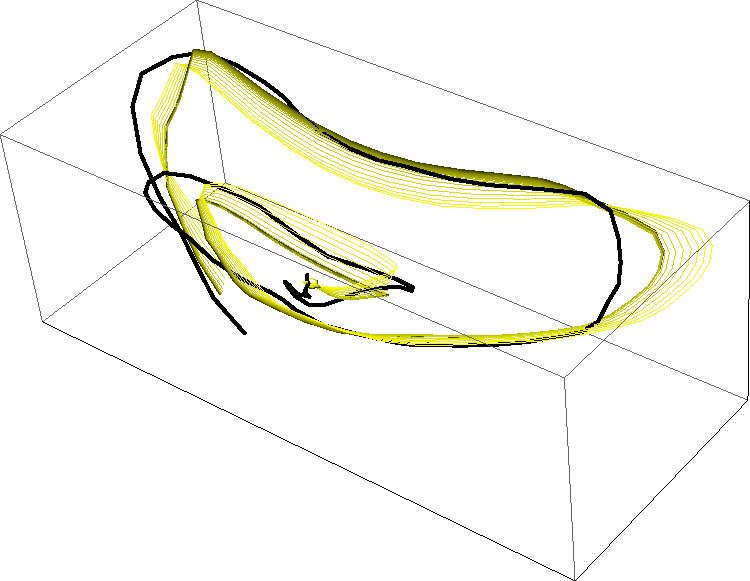
\includegraphics[width = 160pt]{paths12.pdf}
\caption{The path the robot's end effector took through space.  The black line is the measured end effector's path while the yellow lines are the end effector's simulated path for each iteration of the steepest descent algorithm.  The iteration numbers are ordered from lighter yellow to darker yellow.  }
\label{fig-paths}
\end{figure}

Loop back to challenges from First section
\begin{enumerate}
  \item Integrate touch with visual sensors.
  \item Where/how to initially grip the object.
  \item Multiple grip locations and multiple tests for identification.
  \item Multiple arms.
  \item Additional stimuli like external forces that are due to other objects than the one of consideration---for example, working in a cluttered environment.
  \item Choosing manipulator trajectories that provide the most information.
  \item Unknown topology or geometry.
  \item Choosing the model discretization that best balances model fidelity with computation speed.
  \item Stable manipulation while maintaining fidelity of parameter optimization.
  \item Updating identification for systems that will change over long time horizon's---for example plant growth over full life cycle.
\end{enumerate}

\newpage
\bibliographystyle{plain}
\bibliography{param_opts_cites}

\end{document}
